\documentclass[tikz]{standalone}
\usepackage{../../sty/tikz_preamble}
\begin{document}

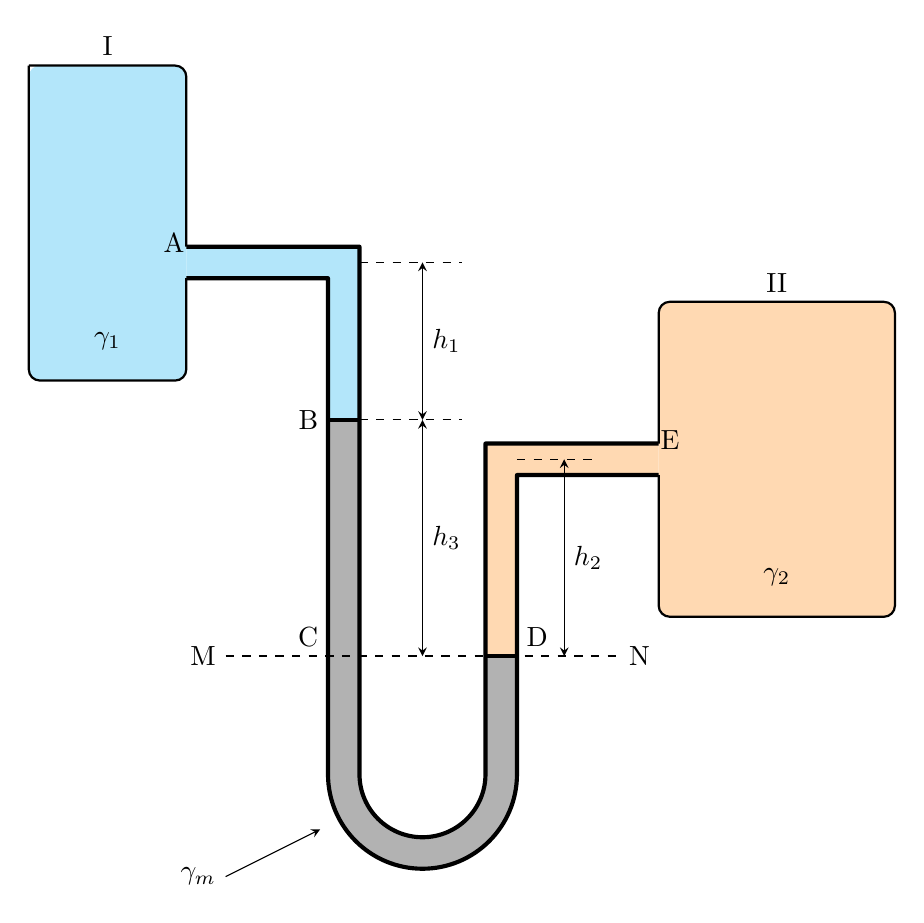
\begin{tikzpicture}[>=stealth,
  contorno/.style={line width=1.5pt, draw=black, line join=round}]
  \colorlet{fluid1}{cyan!30}
  \colorlet{fluidm}{gray!60}
  \colorlet{fluid2}{orange!30}
  \fill[fluid1, rounded corners] (-1, 4.5) rectangle (1, 8.5);
  \fill[fluid1] (1, 5.8) -- (2.8, 5.8) -- (2.8, 4) -- (3.2, 4) --
  (3.2, 6.2) -- (1, 6.2) -- cycle;
  \fill[fluidm]
  (2.8, 4) -- (3.2, 4) -- % Interfaz B
  (3.2, -0.5) arc(180:360:0.8) -- % Curva interior del tubo en U
  (4.8, 1) -- (5.2, 1) -- % Interfaz D
  (5.2, -0.5) arc(360:180:1.2) -- % Curva exterior del tubo en U
  cycle;

  \fill[fluid2, rounded corners] (7, 1.5) rectangle (10, 5.5);
  \fill[fluid2] (4.8, 1) -- (5.2, 1) -- (5.2, 3.3) -- (7, 3.3) -- (7,
  3.7) -- (4.8, 3.7) -- cycle;
  \draw[thick, rounded corners] (-1, 8.5) -- (-1, 4.5) -- (1, 4.5) -- (1, 5.8);
  \draw[thick, rounded corners] (1, 6.2) -- (1, 8.5) -- (-1, 8.5);
  \draw[thick, rounded corners] (7, 3.3) -- (7, 1.5) -- (10, 1.5) --
  (10, 5.5) -- (7, 5.5) -- (7, 3.7);
  \draw[thick,contorno] (1, 6.2) -- (3.2, 6.2) -- (3.2, -0.5)
  arc(180:360:0.8) -- (4.8, 3.7) -- (7, 3.7);
  \draw[thick,contorno] (1, 5.8) -- (2.8, 5.8) -- (2.8, -0.5)
  arc(180:360:1.2) -- (5.2, 3.3) -- (7, 3.3);
  \draw[thick,contorno] (2.8, 4) -- (3.2, 4); % Nivel B
  \draw[thick,contorno] (4.8, 1) -- (5.2, 1); % Nivel D
  \draw[dashed, thick] (1.5, 1) -- (6.5, 1);
  \node[left] at (1.5, 1) {M};
  \node[right] at (6.5, 1) {N};
  \draw[dashed] (3.2, 6) -- (4.5, 6);   % Nivel A (centro del tubo izquierdo)
  \draw[dashed] (3.2, 4) -- (4.5, 4);   % Nivel B
  \draw[dashed] (5.2, 3.5) -- (6.2, 3.5); % Nivel E (centro del tubo derecho)
  \draw[<->] (4, 4) -- (4, 6) node[midway, right] {$h_1$};
  \draw[<->] (4, 1) -- (4, 4) node[midway, right] {$h_3$};
  \draw[<->] (5.8, 1) -- (5.8, 3.5) node[midway, right] {$h_2$};
  \node[above left] at (1.1, 6) {A};
  \node[left] at (2.8, 4) {B};
  \node[above left] at (2.8, 1) {C};
  \node[above right] at (5.2, 1) {D};
  \node[above right] at (6.9, 3.5) {E};
  \node[above] at (0, 8.5) {I};
  \node[above] at (8.5, 5.5) {II};
  \node at (0, 5) {$\gamma_1$};
  \node at (8.5, 2) {$\gamma_2$};
  \draw[<-] (2.7, -1.2) -- (1.5, -1.8) node[left] {$\gamma_m$};
\end{tikzpicture}
\end{document}
